\documentclass[12pt,a4paper]{article}
\usepackage[czech]{babel}
\usepackage[utf8]{inputenc}
\usepackage[T1]{fontenc}
\usepackage{graphicx}
\usepackage{amsmath}
\usepackage{hyperref}
\usepackage[margin=2cm]{geometry}

\title{Semestrální práce: Automatické prahování obrazu \\ Metody Otsu a Sauvola}
\author{Jan Čácha}
\date{\today}

\begin{document}

% Titulní strana
\begin{titlepage}
    \centering
    {\LARGE\bfseries Vysoká škola \\[0.3cm]}
    {\Large Fakulta aplikovaných věd\\[2cm]}
    
    {\Huge\bfseries Semestrální práce\\[1cm]}
    {\LARGE Automatické prahování obrazu\\[0.5cm]}
    {\Large Metody Otsu a Sauvola\\[2cm]}
    
    \begin{tabular}{rl}
        Autor: & Jan Čácha \\
        Studijní program: & Informatika \\
        Předmět: & Zpracování vizuální informace \\
        Akademický rok: & 2024/2025 \\
    \end{tabular}
    
    \vfill
    {\large \today}
\end{titlepage}

% Obsah
\tableofcontents
\thispagestyle{empty}
\newpage

\setcounter{page}{1}

\section*{Abstrakt}
Tato práce se zabývá implementací dvou metod automatického prahování obrazu - Otsuovy metody a Sauvolova adaptivního prahování. Vytvořili jsme aplikaci v Pythonu s grafickým rozhraním, která umožňuje experimentální porovnání těchto metod. Práce obsahuje teoretický rozbor, popis implementace a diskuzi výsledků.

\section{Úvod}
Prahování je základní operace v digitálním zpracování obrazu používaná pro separaci objektů od pozadí. Cílem této práce je:

\begin{itemize}
\item Implementovat Otsuovu metodu (globální prahování)
\item Implementovat Sauvolovu metodu (lokální adaptivní prahování)
\item Vytvořit uživatelsky přívětivé GUI pro experimentování
\item Vyhodnotit výhody a nevýhody obou metod
\end{itemize}

\section{Teoretický rozbor}

\subsection{Otsuova metoda}
Metoda navržená Nobuyukim Otsuem v roce 1979 hledá optimální prah maximalizací mezitřídního rozptylu.

Matematický základ:

\begin{equation}
\sigma_b^2(t) = w_0(t) \cdot w_1(t) \cdot [\mu_0(t) - \mu_1(t)]^2
\end{equation}

Kde:
\begin{itemize}
\item $w_0, w_1$ jsou pravděpodobnosti tříd
\item $\mu_0, \mu_1$ jsou střední hodnoty tříd
\item $t$ je testovaný práh
\end{itemize}

\subsection{Recursive Otsu metoda}
Rozšíření klasické Otsuovy metody \cite{nina2010recursive} řešící problémy s:

\begin{itemize}
\item Slabými tahy písma (faint strokes)
\item Prosakováním z druhé strany (bleed-through)
\item Nerovnoměrným osvětlením (non-uniform illumination)
\end{itemize}

Algoritmus pracuje v těchto krocích:

\begin{enumerate}
\item Odhad pozadí pomocí medianového filtru (velikost okna 21×21)
\item Odstranění pozadí subtrakcí
\item Bilateralní filtrace pro redukci šumu ($\sigma_s=10$, $\sigma_r=2$)
\item Rekurzivní prahování:
\begin{equation}
T_k = \text{Otsu}(T_{k-1}, 255) \quad \text{s kritérii zastavení } d_1=2, d_2=26
\end{equation}
\item Selektivní bilateralní filtrace (odlišné parametry pro text a pozadí)
\item Prahování s hysterezí
\end{enumerate}

Klíčovou inovací je rekurzivní aplikace Otsuovy metody na postupně se zužující intenzitní rozsah, což umožňuje zac

\subsection{Sauvolova metoda}
Adaptivní metoda vyvinutá Sauvolou a Pietikäinenem počítá lokální práh podle vzorce:

\begin{equation}
T(x,y) = \mu(x,y) \left[ 1 + k \left( \frac{\sigma(x,y)}{R} - 1 \right) \right]
\end{equation}

Parametry:
\begin{itemize}
\item $k$ - citlivost na kontrast (0.1-0.5)
\item $R$ - normalizační konstanta (typicky 128)
\end{itemize}

\section{Implementace}

\subsection{Použité technologie}
\begin{itemize}
\item Python 3 s knihovnami: OpenCV, NumPy, PIL
\item Tkinter pro grafické rozhraní
\item Matplotlib pro zobrazování histogramů
\end{itemize}

\subsection{Klíčové algoritmy}

\subsubsection{Otsuovo prahování}
\begin{verbatim}
def otsu_threshold(image):
    hist = np.histogram(image, bins=256)[0]
    prob = hist / hist.sum()
    max_var, optimal = 0, 0
    for t in range(1,256):
        w0, w1 = prob[:t].sum(), prob[t:].sum()
        mu0 = (np.arange(t)*prob[:t]).sum()/w0
        mu1 = (np.arange(t,256)*prob[t:]).sum()/w1
        var = w0*w1*(mu0-mu1)**2
        if var > max_var:
            max_var, optimal = var, t
    return optimal
\end{verbatim}

\subsubsection{Sauvolovo prahování}
\begin{verbatim}
def sauvola(image, window=15, k=0.2, R=128):
    pad = window//2
    padded = np.pad(image, pad, mode='reflect')
    result = np.zeros_like(image)
    for i in range(image.shape[0]):
        for j in range(image.shape[1]):
            window = padded[i:i+window,j:j+window]
            mean, std = window.mean(), window.std()
            T = mean*(1 + k*(std/R - 1))
            result[i,j] = 255 if image[i,j] > T else 0
    return result
\end{verbatim}

\subsubsection{Rekurzivní Otsu}
\begin{verbatim}
def recursive_otsu(image, levels=3, d1=2, d2=26):
    thresholds = []
    prev_thresh = 0
    for _ in range(levels):
        current_image = image if not thresholds else image[image >= prev_thresh]
        thresh = otsu_threshold(current_image)
        if thresholds and (thresh-prev_thresh < d1 or thresh-prev_thresh > d2):
            break
        thresholds.append(thresh)
        prev_thresh = thresh
    return thresholds
\end{verbatim}

\subsubsection{Selektivní bilateralní filtrace}
\begin{verbatim}
def selective_bilateral_filter(image, mask):
    fg = cv2.bilateralFilter(image, -1, 2, 2)  # Konzervativní pro text
    bg = cv2.bilateralFilter(image, -1, 10, 3) # Agresivnější pro pozadí
    return np.where(mask > 0, fg, bg)
\end{verbatim}

\section{Výsledky}


\begin{table}[h]
\centering
\caption{Porovnání metod}
\begin{tabular}{|l|l|l|}
\hline
Metoda & Výhody & Nevýhody \\
\hline
Otsu & Rychlá, dobrá pro bimodální histogram & Špatně pracuje s nerovnoměrným osvětlením \\
Recursive Otsu & Zachycuje slabé tahy, robustní k degradaci & Náročnější na výpočet \\
Sauvola & Adaptivní k místním podmínkám & Pomalá výpočetně náročná \\
\hline
\end{tabular}
\end{table}
\newpage
\begin{figure}[h]
\centering
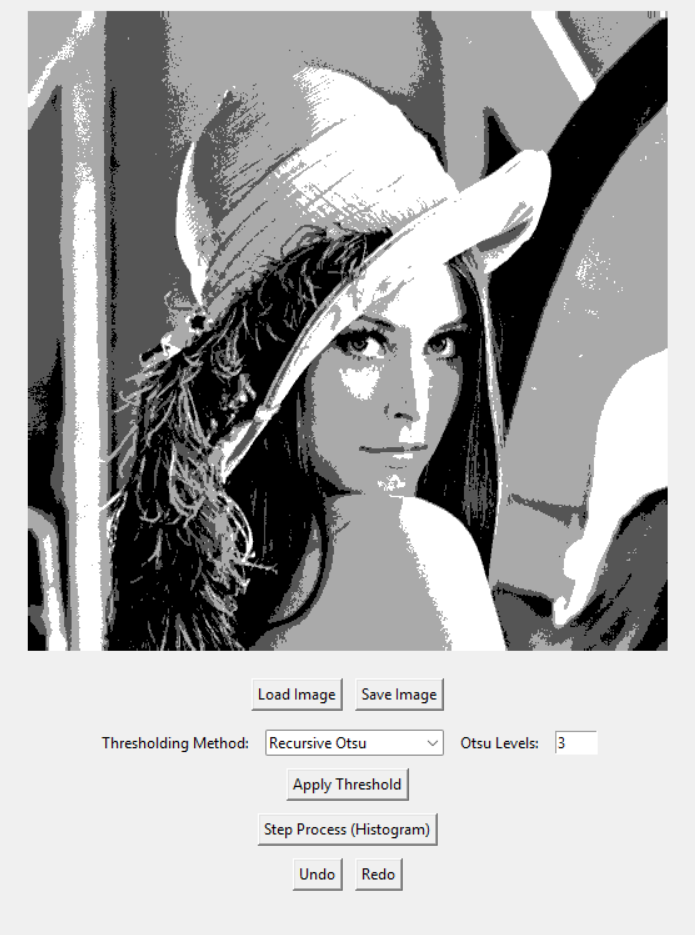
\includegraphics[width=0.8\textwidth]{otsu.png}
\caption{Příklad prahování Recursive Otsu}
\label{fig:vysledky}
\end{figure}


\section{Uživatelská příručka}

\subsection{Instalace}
\begin{enumerate}
\item Instalace Pythonu 3.8 nebo novějšího z \url{https://www.python.org/downloads/}
\item Instalace potřebných knihoven:
\begin{verbatim}
pip install opencv-python numpy pillow matplotlib scikit-image
\end{verbatim}
\item Stažení zdrojového kódu aplikace z repozitáře:
\begin{verbatim}
https://github.com/Lucky01dot/ZVI-Thresholding-RecursiveOtsu-Sauvola.git
\end{verbatim}
\end{enumerate}

\subsection{Spuštění aplikace}
\begin{verbatim}
ZVI-Thresholding-RecursiveOtsu-Sauvola
python threshold.py
\end{verbatim}

\subsection{Popis rozhraní}


Aplikace obsahuje následující ovládací prvky:

\subsubsection{Horní panel}
\begin{itemize}
\item \textbf{Načíst obrázek} - Tlačítko pro výběr vstupního obrázku (formáty: PNG, JPG, BMP)
\item \textbf{Uložit obrázek} - Uložení výsledku prahování
\end{itemize}

\subsubsection{Střední část}
\begin{itemize}
\item \textbf{Zobrazovací panel} - Zobrazuje původní a upravený obrázek
\item \textbf{Undo/Redo} - Vrácení nebo obnovení předchozí operace
\end{itemize}

\subsubsection{Nastavení prahování}
\begin{itemize}
\item \textbf{Metoda}:
\begin{itemize}
\item Otsu - Globální metoda s volbou počtu úrovní (2-4)
\item Sauvola - Lokální metoda s nastavením:
  \begin{itemize}
  \item Velikost okna (liché číslo $\geq$ 3)
  \item Parametr k (0.1-0.5)
  \item Parametr R (doporučeno 128)
  \end{itemize}
\end{itemize}
\item \textbf{Histogram} - Zobrazení histogramu aktuálního obrázku
\end{itemize}

\subsection{Postup práce}
\begin{enumerate}
\item Načtěte vstupní obrázek pomocí tlačítka \textit{Načíst obrázek}
\item Zvolte metodu prahování:
\begin{itemize}
\item Pro Otsu: Nastavte počet úrovní (pro binární prahování zvolte 2)
\item Pro Sauvola: Experimentujte s velikostí okna a parametry k, R
\end{itemize}
\item Klikněte na \textit{Aplikovat prahování}
\item Prohlédněte si výsledek a v případě potřeby upravte parametry
\item Pro zobrazení histogramu klikněte na \textit{Histogram}
\item Výsledek uložte pomocí \textit{Uložit obrázek}
\end{enumerate}

\subsection{Řešení problémů}
\begin{itemize}
\item \textbf{Chybějící knihovny}: Spusťte příkaz pro instalaci knihoven
\item \textbf{Pomalé zpracování}: Pro Sauvolovu metodu zvolte menší okno
\item \textbf{Špatné výsledky}:
\begin{itemize}
\item U Otsu: Zkontrolujte, zda má obrázek bimodální histogram
\item U Sauvola: Upravte parametr k (zvýšit pro nízký kontrast)
\end{itemize}
\item \textbf{Nefungují tlačítka Undo/Redo}: Operace se ukládají až po dokončení
\end{itemize}

\subsection{Doporučené parametry}
\begin{table}[h]
\centering
\caption{Doporučené hodnoty parametrů}
\begin{tabular}{|l|l|l|}
\hline
Typ obrazu & Metoda & Parametry \\
\hline
Dobře osvětlený dokument & Otsu & Úrovně: 2 \\
Dokument s nerovnoměrným osvětlením & Sauvola & Okno: 15-25, k=0.3, R=128 \\
Obrázek s šumem & Sauvola & Okno: 15, k=0.2, R=64 \\
\hline
\end{tabular}
\end{table}

\section{Závěr}
Práce úspěšně implementovala obě metody prahování. Z výsledků vyplývá:
\begin{itemize}
\item Otsuova metoda je vhodná pro obrazy s rovnoměrným osvětlením
\item Sauvolova metoda lépe zpracovává reálné dokumenty
\item GUI aplikace umožňuje snadné experimentování
\end{itemize}

Možná vylepšení:
\begin{itemize}
\item Optimalizace Sauvolovy metody pomocí integrálních obrazů
\item Přidání dalších metod prahování
\end{itemize}

\section*{Literatura}
\begin{enumerate}
\item Otsu, N. (1979). A Threshold Selection Method from Gray-Level Histograms
\item Sauvola, J. (2000). Adaptive Document Image Binarization
\item Gonzalez, R. C. (2008). Digital Image Processing
\item Nina, O., Morse, B., Barrett, W. (2010). \textit{A Recursive Otsu Thresholding Method for Scanned Document Binarization}. Brigham Young University.
\end{enumerate}

\end{document}